\section{Architecture}

\subsection{Architecture}
\begin{frame}
    \frametitle{Architecture}
	\begin{figure}
		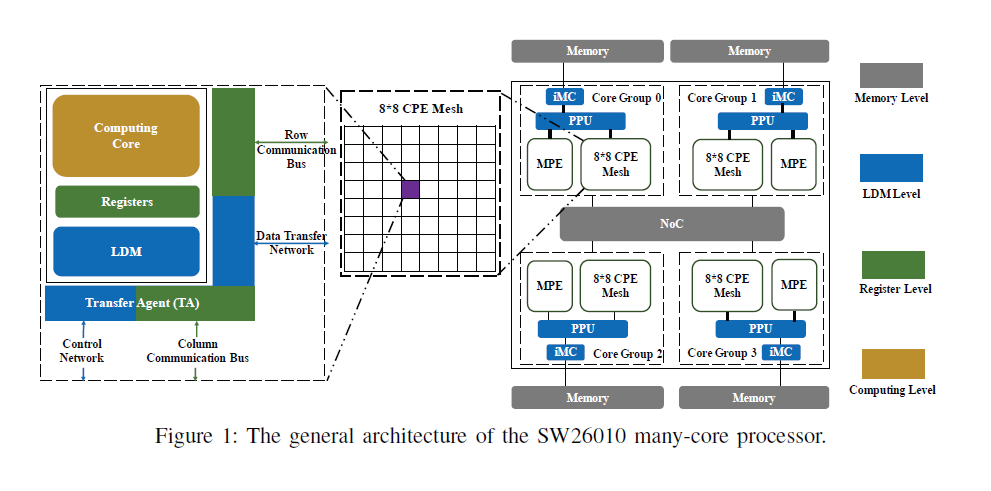
\includegraphics[scale=0.4]{figure/archi.PNG}
	\end{figure} 
\end{frame}

\subsection{Unique features}
\begin{frame}
    \frametitle{Unique features}
	\begin{itemize}
		\item Each CG has an MPE.
		\item Users can explicitly set the sizeof each CG's private memory space, and the size of shared memory space.  
		\item Support a 64kb user-controlled fast buffer for each computing cores. 
		\item Rigister communication between computing cores.
		\item Each computing core consists of two execution pipelines.  
	\end{itemize} 
\end{frame}

\subsection{Challenges}
\begin{frame}
    \frametitle{Challenges}
	\begin{itemize}
		\item Low memory bandwidth. 
		\begin{itemize}
			\item SW26010:36 GB/s for each CG, 144 GB/S for entire processor.  
			\item NVIDIA K80GPU: 480 GB/S for entire processor. 
		\end{itemize}
		\item CPEs do not have a shared buffer to rely on a fine-grained data sharing scheme. 
	\end{itemize}
\end{frame}

	

